\documentclass[a4paper, 12pt]{article}
\usepackage[left=1.5cm, text={18cm, 25cm}, top=2.5cm]{geometry}
\usepackage[utf8]{inputenc}
\usepackage[czech,english]{babel}
\usepackage{cite}
\usepackage{graphicx}
\usepackage{float}
\usepackage{amsmath}
\usepackage{amssymb}
\usepackage{tikz}
\usepackage{url}
\usepackage{comment}
\usepackage[longend,ruled,vlined,commentsnumbered,linesnumbered]{algorithm2e}
\newcommand{\myuv}[1]{\quotedblbase #1\textquotedblleft}
\let\oldnl\nl% Store \nl in \oldnl
\newcommand{\nonl}{\renewcommand{\nl}{\let\nl\oldnl}}% Remove line number for one line

\title{Simulation of non-deterministic finite tree automata}
\author{Martin Hruška, Petr Šebek\\\{xhrusk16, xsebek02\}@stud.fit.vutbr.cz}

\date{}
\begin{document}

\maketitle

\section{Introduction}
\label{sec:intro}

Non-deterministic finite tree automata (NTA) is formalism often used in the field of formal verification.
For example, it can be used for shape analysis of programs manipulating complex data structure where
state of heap is represented by a set of the tree automata \cite{methods12}.
The mentioned technqiue is based on the framework of abstract interpretation where one of fundamentals
operations is computing fixed point (mainly for the cycles in a program) what includes checking inclusion of
tree automata languages.
Checking inclusion is easy for deterministic tree automata (DTA) but much harder for NTA because
na{\"i}ve algorithm has exponential complexity.
It is not also possible to use DTA in these techniques because NTA can represent same language in much more
conciser way and determinization could lead to exponential grow of the  number of the states.
However, there are efficient algorithms for checking language inclusion (based on antichains introduced in \cite{tacas10})
with which it is possible to make more efficient by computing simulation relation over the states of checked automata \cite{tacas10}.
Simulation reduce state space which is needed to explore to check whether inclusion holds.
On the other side, computation of simulation relation has itself cubic complexity so the time needed
to compute it is sometimes bigger than saved state space.
This leads to need of trying the new methods for computing simulation which can be more efficient and
reduce its complexity to level when it will be efficient enough to be used always for enhancing inclusion checking. 

Being more general, simulation relation is attribute of graphs not only automata \cite{focs95, tacas08}.
In case of tree automata it is possible to compute upward or downward simulation but in this
work we consider only downward simulation.
As we mentioned earlier simulation brings reduction of states which we need explore performing
certain algorithms over tree automata because it often holds that when state $p$ is simulated by $q$
we don't further explore state $p$.
Moreover, it is possible also to perform reduction of states of a NFA by computing
equivalence classes on simulation relation and merging states in a same class.

Another technique dealing with complexity of NFA is their representation using mutli-terminal binary decision diagrams (MTBDD).
The symbols of a NFA are encoded to binary representation so the transitions can represented by shared MTBDD what is very efficient mainly for NFA with large alphabeth
(in the second possible representation -- symbols are represented explicitly for each transition).
A~NFA could be represented in bottom-up way or top-down way by MTBDD, in this work we consider only top-down way.

In this work we would like to combine straightforwardness of implementation of simulation over explicitly
represented tree automata and conciser representation of automata by MTBDD.
We suppose NTA represented by MTBDD and we will compute simulation by it conversion
to explicit one with gradual reduction of number of the NFA symbols.
We use computed simulation for more efficient inclusion computation and evaluate whether the method brings any advantage.
The implementation is realized as an extension of VATA library which is state-of-the-art library for NTA manipulation.

In Section \ref{sec:analysis} we give formal definitions, in Section \ref{sec:bdd} MTBDD representation of automata is described.
Section \ref{sec:bdd} describes VATA library, Section \ref{sec:vata} provides description of design of our solution.
Implementation details take place in Section \ref{sec:impl} and finally experiments are evaluated in Section \ref{sec:exps}.

\section{Preliminaries}
\label{sec:analysis}
In this section NTA and simulation over NTA states will be defined more formally.

A~\emph{ranked alphabeth} is a finite set of symbols $\Sigma$ associated with a mapping $\#: \Sigma \rightarrow \mathbb{N}_0$
that assigns ranks to symbols. A~\emph{tree} is a graph $t$ which is either empty or it has exactly one root and each of its
nodes is the $i$-th successor of at most one node $v$ for some $i \in \mathbb{N}_0$

A~\emph{finite, non-deterministic, top-down tree automata} is a quadratuple $A=(Q, \Sigma, \delta, R)$ where
$Q$ is a finite set of \emph{states}, $R\subseteq Q$ is a set of \emph{root states}, $\Sigma$ is a ranked alphabeth,
$\delta$ is a set of the transition rules.
Each transition is a triple of the form $(q,a,q_1, \ldots, q_n)$ where $n \geq 0$, $q, q_0 \ldots q_n \in Q$, $a \in \Sigma$ and $\#(a) = n$.
When $n = 0$ then such a transition is called a \emph{leaf rules}.
A~\emph{bottom-up} automaton is a quadratuple $B=(Q, \Sigma, \delta, F)$, where $Q$, $F$ are same as for $top-down$ automaton, $F\subseteq Q$
is a set of final states and $\delta$ is a transition relation with rules which are in the form $(q_1,\ldots, q_n,a,q)$ where $n \geq 0$ and $\#(a) = n$.
We can interchange the two notations because non-deterministic automata are known to have same expressive power in bottom-up and top-down version \cite{tata}.

[TODO: maybe define semantics of TA]


For a bottom-up NTA $A=(Q, \Sigma, \delta, R)$, a \emph{downward simulation} $\preceq\, \subseteq Q\times Q$ is binary relation such that $q \preceq p$
and $(q,a,q_1,\ldots, q_n),a,q)$ then $\exists (p_1, \ldots, p_n) \rightarrow p \wedge \forall i \in {1 \ldots n}: q_i \preceq p_i$.

\section{BDD representation}
\label{sec:bdd}

This section is based on~\cite{fiedor:wsks}. \textit{Reduced ordered binary decision diagram} (ROBDD) is directed acyclic graph with single \textit{source} node called \textit{root} and at least two \textit{sink} nodes 0 and 1. Nodes that are not sink nodes are called \textit{internal nodes}. ROBDD are defined over a set of $n$ Boolean variables $X = \{x_1, \dots, x_n\}$, we assume that $X$ can be ordered: $x_1 < x_2 < \dots < x_n$. Now for each internal node $v$, there exists two outgoing edges with label \textit{low} and \textit{high}. We further can define function \textit{var} which assign Boolean variables to the internal nodes of ROBDD. In ROBDDs there holds next condition: $var(v) < var(v.low) \wedge var(v) < var(v.high) \wedge v.low \neq v.high$, thus successor has always higher value. ROBDD nodes therefore represent $n$-ary Boolean functions that map each assignment to the Boolean variables in $X$.

\textit{Mutli-terminal binary decision diagram} (MTBDD) is then ROBDD generalized to more than two sink nodes. Further we can define \textit{shared} MTBDD, MTBDD with multiple source nodes/roots. You can see difference between ordinary BDD and MTBDD in Figure \ref{fig:15860}.

\begin{figure}[h]
	\centering
	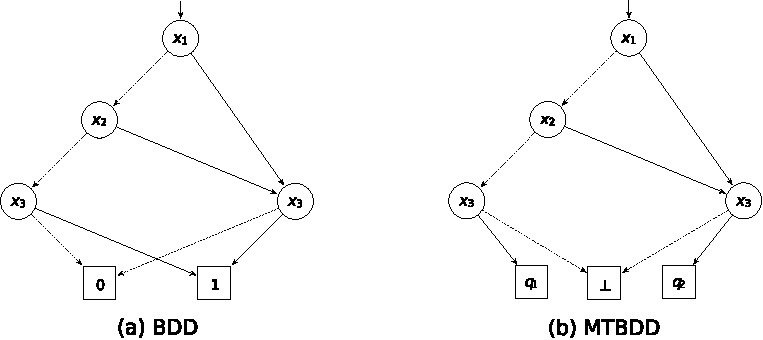
\includegraphics[width=0.7\linewidth]{15860.pdf}
	\caption{Comparison of ROBDD and MTBDD \cite{fiedor:wsks}}
	\label{fig:15860}
\end{figure}

Let $A=(Q, \Sigma, \delta, R)$ be a tree automaton. We can encode symbols to binary sequence with some function $enc: \Sigma \rightarrow \{0, 1\}^n$, for some $n$. Each position $1\leq i \leq n$ is then assigned a Boolean variable from set $X = \{x_1, \dots, x_n\}$. We define $Q^\#$ as set of all tuples of states from $Q$ with up to the maximum arity that some symbol in $\Sigma$ has.

Finally we can define \textit{top-down} representation of the transition function $\delta$ of the TA $A$ uses a shared MTBDD $\delta^{td}$ over $\Sigma$, where the set of roots $R=Q$ and the domain of labels of sink nodes is $2^{Q^\#}$. MTBDD $\delta^{td}$ then represents the function
\begin{equation*}
[[ \delta^{td}]]  : Q \rightarrow (\Sigma \rightarrow 2^{Q^\#}t)
\end{equation*}
\begin{equation*}
[[ \delta^{td}]]   = \lambda q a . \{(q_1, \dots, q_p) | q \xrightarrow{a} (q_1, \dots, q_p) \} 
\end{equation*}

As an example we can take TA with following transitions:
\begin{alignat*}{4}
q_1 \xrightarrow{00\overline{X}} q_1, \qquad &
q_1 \xrightarrow{011} q_1, \qquad & 
q_1 \xrightarrow{110} q_1, \qquad &
q_1 \xrightarrow{10\overline{X}} q_1, \qquad & \\
q_1 \xrightarrow{010} q_1, \qquad &
q_1 \xrightarrow{111} q_1, \qquad &
q_1 \xrightarrow{\overline{X}\overline{X}\overline{X}} q_2 \qquad &  &\\
\end{alignat*}

Where symbol $\overline{X}$ denotes either 0 or 1. MTBDD encoding this transition is depicted at Figure~\ref{fig:MTBDD}.

\begin{figure}[h]
\centering
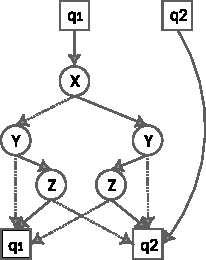
\includegraphics[width=4cm]{MTBDD}
\caption{Example of MTBDD representing automaton transitions}
\label{fig:MTBDD}
\end{figure}


\section{VATA}
\label{sec:vata}
VATA is library for efficient manipulation with NTA \cite{libvata}.
It provides both encoding for NTA -- semi-symbolic via MTBDD and explicit which will be described further.
VATA is open-source licensed under GPL license and it is written in C++.
It currently supports TIMBUK as input format.

The main goal of VATA is to provide state-of-the-art algorithms for inclusion checking
but it also contains implementation of standard operations like union or intersection.
As we mentioned in Section \ref{sec:intro} inclusion checking is related to simulation
since simulation relation could bring more efficiency to the state-of-the-art algorithms like antichains \cite{tacas10}.
There are already implemented algorithms for computing simulation in VATA but not one of them uses method which we used.
The algorithms for simulation computing in VATA uses encoding to LTL systems \cite{tacas08} in case of explicit encoding
and there are some implementations over MTBDD which are not known to work at all.

\subsection{Explicit representation}

The explicitly represented automaton is represented by its transition set using two hash maps.
The first one maps each state $q$ to the second hash map which maps symbol $a$ set of tuples $(q_1,\ldots,q_n)$ for all $a(q_1, \ldots, q_n) \rightarrow q \in \delta$.
The set of states is not stored explicitly because it is possible to obtain it from transition relation.
However, a set of final states is represented like a standard set.

\subsection{Semi-Symbolic Representation}

Semi-symbolic representation is based on representing transition relation using MTBDD.
The particular details of encoding of a NTA to MTBDD is described in section \ref{sec:bdd}.
The VATA library provides two possible MTBDD representation -- top-down and bottom-up.
The first one stores MTBDD for each $q \in Q$ and all transition where $q$ is on right-handed side
are represented by the MTBDD.
The MTBDD terminal symbols are sets of tuples which it is possible to make transition from $q$ to.
The bottom-up representation inversely, MTBDD exists for each tuple of the NTA and MTBBD represents all transitions with
the tuple on left-handed side and the terminal symbols are sets of states which it is possible to make transition to.

\section{Design}
\label{sec:design}

This section describes conceptual design of our method for computing simulation and related algorithms.
For implementation details please see Section \ref{sec:impl}.

As the input of our method we take a NTA represented by MTBDD in top-down way
which we translate into a NTA represented explicitly and we also reduce symbols.
This is done by following general method doing reduction of alphabeth and yielding a new NTA.
Let have a NFA $A=(Q, \Sigma, \delta, F)$, a new ranking alphabeth $\Sigma'$ and mapping $f: 2^\Sigma \rightarrow \Sigma'$,
when there is $((a_1(q_1,\ldots,q_n) \rightarrow q) \in \delta \wedge \ldots \wedge (a_n(q_1,\ldots,q_n) \rightarrow q) \in \delta) \wedge
((a_1(r_1,\ldots,r_n) \rightarrow q) \in \delta \wedge \ldots \wedge (a_n(r_1,\ldots,r_n) \rightarrow q) \in \delta)$
such that $a_i \neq a_{i+1}$ for any $i\in \{1..n\}$ then $(\{a_1, \ldots, a_n\}) \rightarrow A) \in f$.
It is also constructed a new NFA $A' = (Q, \Sigma', \delta', F)$ where $Q, F$ are unchanged to $A$ 
and $\Sigma'$ is the new ranked alphabeth obtained by mapping $f$ and $\delta'$ is transition rules set such that
$(a_1(q_1, \ldots, q_n) \rightarrow q) \in \delta \wedge \ldots \wedge (a_n(q_1, \ldots, q_n) \rightarrow q) \in \delta$ and
$ \{a_1,\ldots,a_n\}  \rightarrow A~\in f$ for some $A \in \Sigma'$, then $A(q_1, \ldots, q_n) \rightarrow q) \in \delta$
for all possible tuples $q_1,\ldots,q_n$ [TODO which tuples].
In our case, the input NFA is semi-symbolic represented one and the output NTA is the same automata in explicit representation.
The change of NTA representation is done in level of implementation details and is not directly related to a design of generic algorithm.
The whole method of translation is described again in Algortihm \ref{alg:translate} to provide more easy to follow way of method description.

\begin{algorithm}[h]
\label{alg:translate}
\KwIn{NTA $A=(Q,\Sigma, \delta, F)$}
    \KwOut{NTA $A'=(Q,\Sigma', \delta', F)$}
    $\delta' := \emptyset $\;
    $\Sigma' "= \emptyset $\;
	$f := \emptyset$\;
	\ForEach{$q \in Q$}
    {
		\ForEach{$(q_1,\ldots, q_n)$, such that $(a(q_1, \ldots, q_n)\rightarrow q) \in \delta)$ for any $a\in \Sigma$}
		{
			$S_q := \{ a\in \Sigma \,|\, \exists(a(q_1,\ldots,q_n) \rightarrow q) \in \delta\}$\;
			\ForEach{$(r_1,\ldots, r_n)$, such that $(b(r_1, \ldots, r_n)\rightarrow q) \in \delta)$ for any $a\in \Sigma$}
			{
				$S_r := \{a\in \Sigma \,|\, \exists\, (a(r_1,\ldots,r_n) \rightarrow q) \in \delta\}$\;
				\If{$(S_q \cap S_r \rightarrow A') \not\in f$ for any $A' \in \Sigma'$}
				{
					add $A'$ to $\Sigma'$ such that $A' \not\in \Sigma'$\;
					add $(S_q \cap S_r \rightarrow A')$ to $f$\;
				}
				add $f(S_q \cap S_r)(q_1,\ldots,) \rightarrow q$ to $\delta'$\;
			}
		}
    }
	\Return $A' = (Q, \Sigma', \delta', F)$
\caption{NTA symbol reduction yielding a new NTA}
\end{algorithm}

Finally, we compute downward simulation over explicit NTA by Algorithm \ref{alg:sim}.
\begin{algorithm}[h]
\label{alg:sim}
\KwIn{NTA $A=(Q,\Sigma, \delta, F)$}
	\KwOut{$\preceq \subseteq Q \times Q$}
	\SetKwFunction{main}{main}
	\SetKwProg{main}{}{}{}
    
	$last := \emptyset $\;
    $sim := \emptyset $\;
	\While{$sim \neq last$}
	{
		$last := sim$\;
		\ForEach{Arity $n$ of $\Sigma$}
		{
			\ForEach{$a \in \Sigma$ such that $\#(a) = n$}
			{
				\ForEach{$(q_1,\ldots, q_n)$, such that $(a(q_1, \ldots, q_n)\rightarrow q) \in \delta)$ for any $q \in Q$}
				{
					$temp := \emptyset$\;
					\ForEach{$(r_1,\ldots, r_n)$, such that $(a(r_1, \ldots, r_n)\rightarrow r) \in \delta)$ for any $r \in Q$ and 
					$q_1 \preceq r_1 \wedge \ldots \wedge q_n \preceq r_n$}
					{
						$temp := temp \cup \{r \in Q \,|\, a(r_1,\ldots, r_n) \rightarrow r\}$\;
					}

					$simRefiment(sim, \{q \in Q \,|\, a(q_1,\ldots, q_n) \rightarrow q\}, temp)$\;
				}
			}
		}

	}
	\Return $sim$\;
	\DontPrintSemicolon \nonl\;
	\setcounter{AlgoLine}{0}

	\SetKwFunction{simRefiment}{simRefiment}
	\SetKwProg{refProc}{Function}{}{}
	\nonl \refProc{\simRefiment{$sim$,$lhs$,$rhs$}}
	{
		\ForEach{$q \in lhs$}
		{
			\ForEach{$(q,r) \in sims$}
			{
				\If{$r \notin rhs$}
				{
					remove $(q,r)$ from $sim$ \;
				}
			}
		}
	 }
\caption{Computing simulation on a NTA TODO cite ondra}
\end{algorithm}


\section{Implementation}
\label{sec:impl}

As we mentioned in Section \ref{sec:vata} VATA library already has infrastructure needed for implementation of
our method.
It contains support for parsing input NTA, its semi-symbolic and explicit representation and implemented
state-of-the-art algorithm for inclusion checking.
So we decided to implement our solution as extension of VATA library.
We design our implementation like a stand-alone module which is compiled separately to the rest of library (using CMake building system exploited in VATA).
Module needs just include some headers for knowing interface of VATA classes for NTA representation.

When we focus on implementation of our module itself we use following classes:
\begin{itemize}
	\item \emph{BDDTopDownSimExpl} Class translates MTBDD represented automaton to explicit one with symbol translation
	\item \emph{BDDTopDownSimComputer} Class computes downward simulation over explicit tree automata
\end{itemize}

We exploited following classes from VATA implementation:

\begin{itemize}
	\item \emph{BDDTDTreeAutCore} Class for semi-symbolic representation of NTA using MTBDD.
	\item \emph{ExplicitTreeAutCore} Class for explicit representation of NTA.
	\item \emph{BinaryDiscontRelation} Class for representation of simulation relation.
\end{itemize}

\section{Experiments}
\label{sec:exps}

The experiments should find out how big efficiency brings our method for computing simulation for checking inclusion of the tree automata.
The experiments was done by checking inclusion of language each automaton to other automata with and without simulation
and comparing needed times for checking inclusion depending on the number of states of the automata.
The time for computing simulation was included into the time needed for checking inclusion with simulation
because it is not often possible to reuse once computed simulation.

We ran experiments on automata from VATA test folder. First we ran experiment with automata with number of states from range 0-60. You can see result of this experiment in Figure~\ref{fig:g}. Please note that y axis is in logarithmic scale. Also note that plots are sorted by nosim\_time, run without simulation. Our experiments had timeout 60 seconds. We checked if result of inclusion with simulation correspond with result of run without simulation. We have 100 \% success rate in computing inclusion result, therefore our simulation algorithm is implemented correctly.

All experiments were ran on computer with OS Fedora 20 with CPU Intel Core i5-2520M with available 8 GiB of RAM.

\begin{figure}[h!]
	\centering
	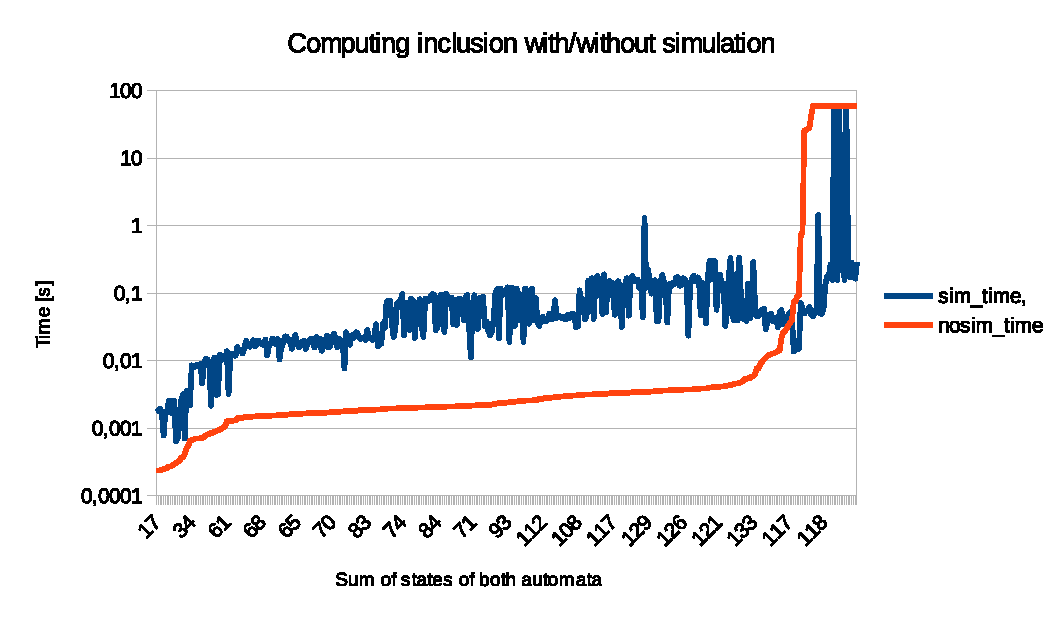
\includegraphics{g}
	\caption{}
	\label{fig:g}
\end{figure}

You can see that variant without simulation runs faster for most of the runs. It is because simulation is demanding per se and only prolong computation time of easily computed inclusions. Easily computed inclusions are those where we can refute inclusion right from start. On the other hand there is a region, where computation with simulation runs considerably slower than without simulation. You can see this region of previous plot in figure~\ref{fig:g_detail}.

\begin{figure}[h!]
	\centering
	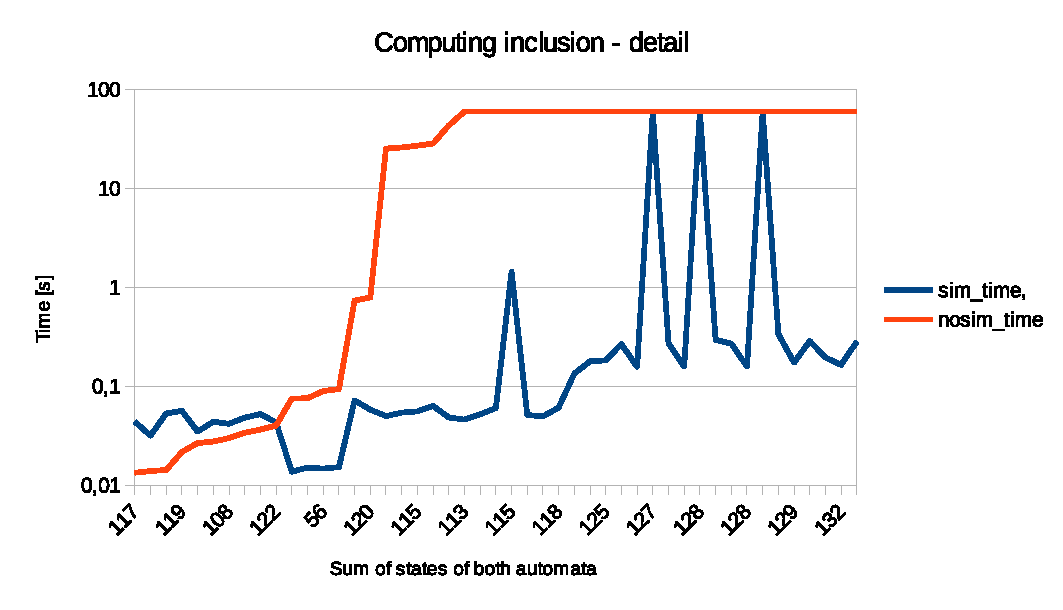
\includegraphics{g_detail}
	\caption{}
	\label{fig:g_detail}
\end{figure}

In this region we reduce some states and simulation runs comparably with previously described problems. This region is what we focus on and is main contribution of this work. For autotama with ~50 states run without simulation can run for ~4 minutes (in environment with disabled timeout) and gets worse with rising number of states. We are able to keep time of computation at ~1 second with simulation, for most cases. As you can see our run is terminated at timeout in some cases too, but in much lower number.

In next experiment we took automata with 110 - 170 states. You can see results of this experiment in figure \ref{fig:g_advanced}. Again you can see that for half cases computation without simulation is faster, but for second half our method  prevails. It still computes its results in 1 second while nosim run is cut off after 60 seconds. We were unable to check time of computation without simulation in these automata because it ran too long.

\begin{figure}[h]
	\centering
	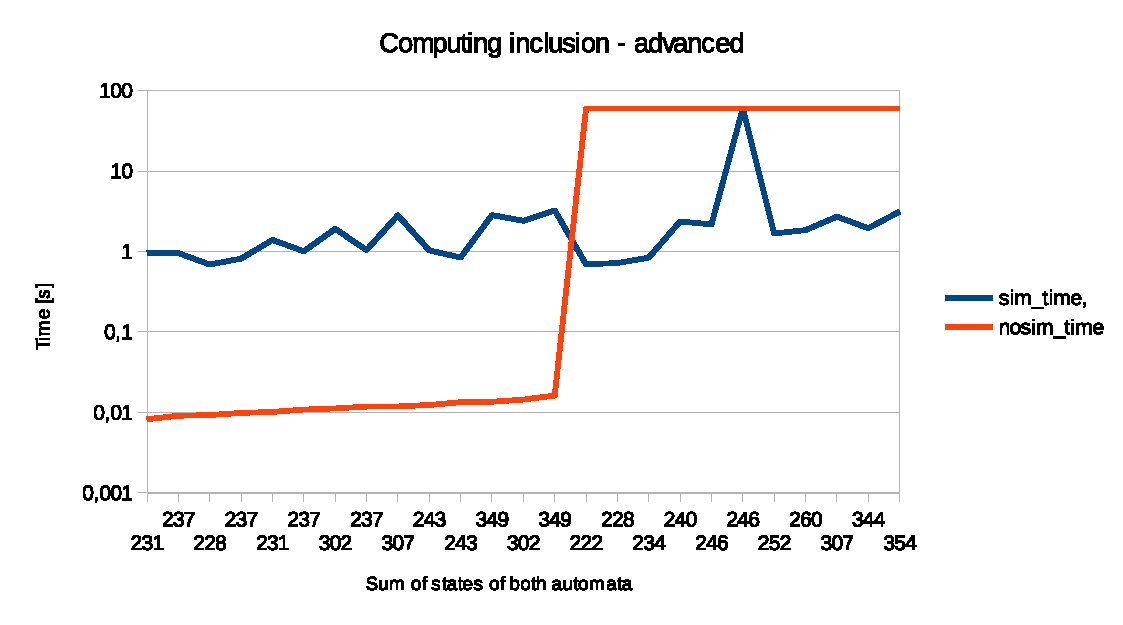
\includegraphics{g_advanced}
	\caption{}
	\label{fig:g_advanced}
\end{figure}

\section{Conclusion}
\label{sec:end}

This work describes implementation of a method for computing simulation over NFA and its implementation.
Our method takes NTA represented in semi-symbolic top-down way using MTBDD, it
turns it to explicit representation and compute downward simulation over it.

We implemented our method as module to VATA library exploiting its infrastructure for manpilationg NTA.
%The method has been evaluated on set of NTA and it has shown that our method and found that it is very awsome.
%It 100000x faster then inclusion checking without simulation
The method has been evaluated on set of NTA and it has shown that our method is justifiable in some cases. It ran 100x faster in these cases. On the other hand for most cases it runs slower than method without simulation because computing simulation is expensive and useless for some cases.


Further research may be done in more efficient manipulation with MTBDD during translation to explicit representation or
extending it to bottom-up automata.
It is also possible to implement NFA reduction which uses computed simulation.

\newpage
\appendix
\section{User guide}
\label{app:usage}

for installation please read README
for run, please read README-gal


\bibliography{literatura}
\bibliographystyle{plain}
\end{document}
